% MTE 481 - Preliminary Design Presentation
% Group 2
%
% A neat PDF slideshow.

%%%%%%%%%%%%
% Preamble %
%%%%%%%%%%%%
\documentclass{beamer}
\mode<presentation>

\usepackage{graphicx}

\title{MTE 481 - Design Project}
\subtitle{Object Avoidance and Navigation for Powered Wheelchairs}
\author{Iain Peet \and Rowan Head-Marsden \and Jordan Valentin}

%%%%%%%%
% Body %
%%%%%%%%
\begin{document}

\begin{frame}
  \titlepage
\end{frame}

\begin{frame}
  \frametitle{Introduction}
  \begin{figure}
    \centering
    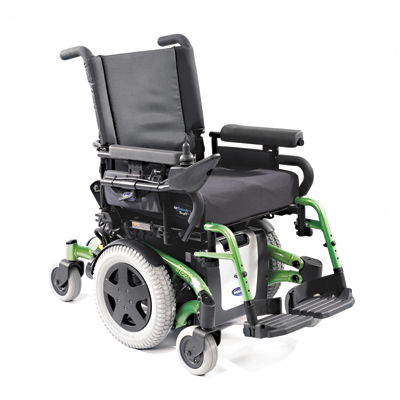
\includegraphics[width=6cm]{wheelchair.jpg} 
  \end{figure}
\end{frame}

\begin{frame}
  \frametitle{Need Statement}
  Powered wheelchairs can improve the mobility of the physically handicapped, but 
  alertness and control are required for safe operation.
  Additional assistive technology is needed in order to afford the same benefits
  to the more severely disabled.
\end{frame}

\begin{frame}
  \frametitle{Objectives \& Constraints}
  \begin{itemize}
    \item Improve the safety of powered wheelchairs, for the occupand and for nearby pedestrians. \\
    \item Make powered wheelchairs accessible to people who would otherwise be denied due to safety concerns. \\
    \item Assist wheelchair users with difficult tasks, such as precise positioning and movement in constrained spaces.  \\
    \item Avoid requiring a specialized, controlled operating environment. \\
    \item It must be possible to integrate with existing wheelchairs. \\
  \end{itemize}
\end{frame}

\begin{frame}
  \frametitle{Criteria}
  \begin{itemize}
    \item Risk of human harm.\\
    \item Tolerance of human error.\\
    \item Robustness against physical damage.\\
    \item Ability to operate in a variety of environments. \\
    \item Price.\\
    \item Electrical power consumption.\\
  \end{itemize}
\end{frame}

\begin{frame}
  \frametitle{Design Concept}
  \begin{itemize}
    \item Use sensor(s) as inputs to a computer-controlled system. \\
    \item Take user input into this system. \\
    \item Combine the user input and sensor readings to determine output to motor controllers. \\
    \item Produce collision-free movement of chair (whether by warnings, automated avoidance, etc.) \\
  \end{itemize}
\end{frame}

\begin{frame}
  \frametitle{Stereo Vision}
  \begin{figure}
    \centering
    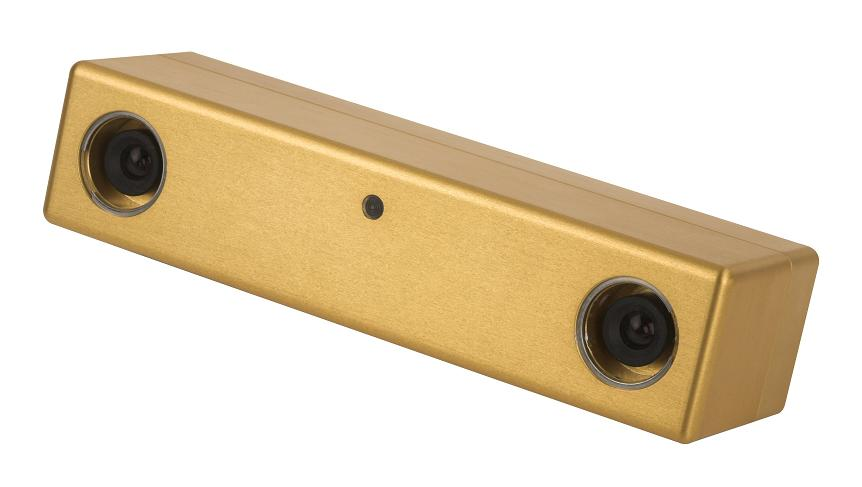
\includegraphics[width=6cm]{stereovision.jpg}
  \end{figure}
\end{frame}

\begin{frame}
  \frametitle{Ultrasonic}
  \begin{figure}
    \centering
    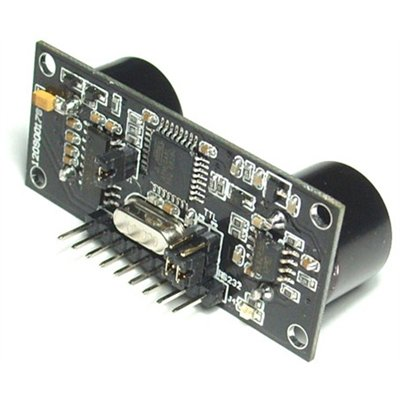
\includegraphics[width=6cm]{ultrasonic.jpg}
  \end{figure}
\end{frame}

\begin{frame}
  \frametitle{Infra-Red}
  \begin{figure}
    \centering
    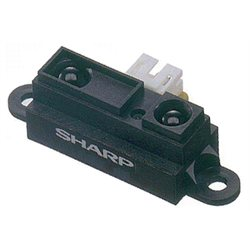
\includegraphics[width=6cm]{ir.jpg}
  \end{figure}
\end{frame}

\begin{frame}
  \frametitle{RADAR}
  \begin{figure}
    \centering
    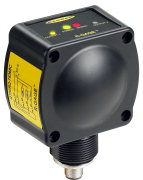
\includegraphics[width=6cm]{radar.jpg}
  \end{figure}
\end{frame}

\begin{frame}
  \frametitle{LIDAR}
  \begin{figure}
    \centering
    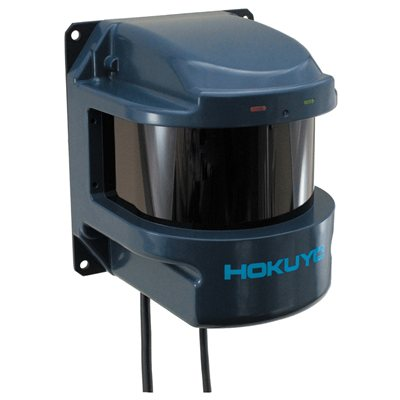
\includegraphics[width=6cm]{laser.jpg}
  \end{figure}
\end{frame}

\begin{frame}
  \frametitle{Microsoft Kinect}
  \begin{figure}
    \centering
    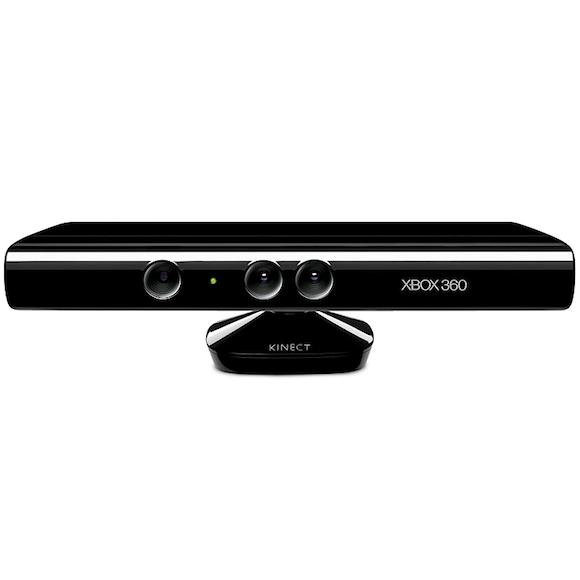
\includegraphics[width=6cm]{Kinect.jpg}
  \end{figure}
\end{frame}

\begin{frame}
  \frametitle{Patent Search}
  ``Computer controlled power wheelchair navigation system''
  \begin{figure}
    \centering
    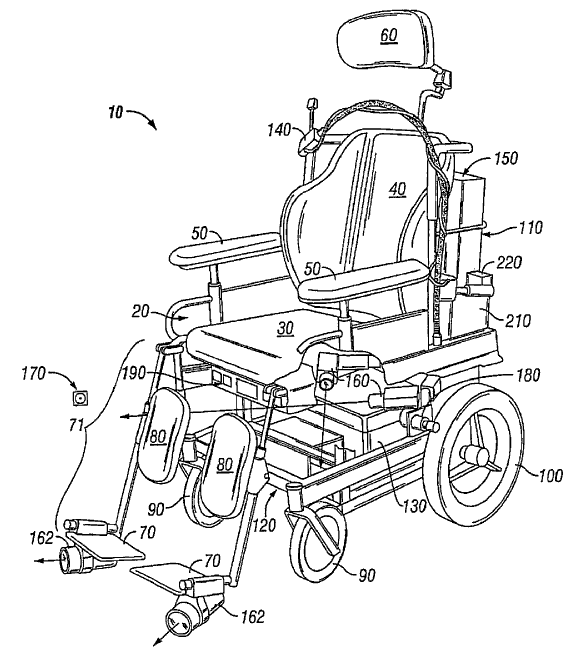
\includegraphics[width=6cm]{patents.png}
  \end{figure}
  \begin{itemize}
    \item Patent No. US 7,383,107 B2 (June 3, 2008) \\
  \end{itemize}
\end{frame}

\begin{frame}
  \frametitle{Patent Search}
  ``Powered Wheelchair''
  \begin{figure}
    \centering
    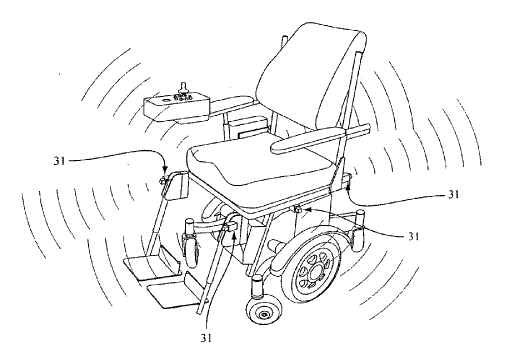
\includegraphics[width=6cm]{patents2.png}
  \end{figure}
  \begin{itemize}
    \item Patent No. US 2010/0082182 A1 (April 1, 2010) \\
  \end{itemize}
\end{frame}

\begin{frame}
  \frametitle{Patent Search}
  ``Wheelchair and method for correcting the guidance of a wheelchair''
  \begin{figure}
    \centering
    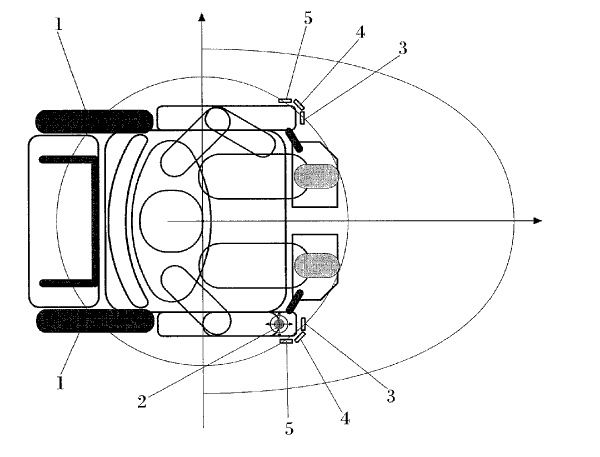
\includegraphics[width=6cm]{patents3.png}
  \end{figure}
  \begin{itemize}
    \item Patent No. US 2011/0130940 A1 (June 2, 2011) \\
  \end{itemize}
\end{frame}

\begin{frame}
  \begin{center}
    \Huge{Questions?}
  \end{center}
\end{frame}


\end{document}
